\section{Misura della polarizzazione}
Ciò che bisogna fissare prima di guardare questo esperimento è che nel decadimento beta di un nucleo che non ha nessuna direzione privilegiata o altro quando decade fissa una direzione e cioè opposta alla direzione del moto degli elettroni. E questo fatto permette di distinguere la desta e la sinistra! Per misurare la polarizzazione di un elettrone occorre chiedersi se ci sono effetti misurabili dipendenti dalla polarizzazione nella interazione di un elettrone o con un campo coulombiano o con un elettrone atomico. Tra i metodi principali abbiamo:
\begin{itemize}
	\item Mott scattering: cioè uno scattering Coulombiano del nucleo di un atomo pesante ma è sensibile solo alla polarizzazione trasversale alla direzione del moto.
	\item M{\o}ller scattering: cioè interazione dell'elettrone che si vuole analizzare con un elettrone atomico ma l'elettrone atomico deve essere polarizzato.
	\item Bhabha scattering: Come il precedente ma per analizzare la polarizzazione di positroni. 
\end{itemize}
Analizzeremo solo un esperimento che usa il primo metodo. Purtroppo lo scattering Coulombiano dipende dalla polarizzazione solo al secondo ordine dell'approssimazione di Born (l'effetto è piccolo: si usano nuclei pesanti e quindi con alto $Z$). Inoltre, come già osservato, è sensibile ad una polarizzazione trasversale.
\section{Rotazione del Vettore di Polarizzazione}
Come trasformare la polarizzazione longitudinale in trasversale? Ovviamente con un campo elettromagnetico. Per descrivere l'effetto di un campo elettromagnetico classico sullo spin di una particella si può utilizzare l'equazione semiclassica (Bergman, Michel, Telegdi)
$$
\hbar \frac{ds^\mu}{d\tau} = 2\mathfrak{m}F^{\mu\nu}s_\nu - 2u^\mu \mathfrak{m}' F^{\nu\lambda}u_\nu s_\lambda
$$
con $\mathfrak{m}=\frac{e\hbar}{2mc}$ è il momento magnetico e $\mathfrak{m}'$ è il momento magnetico anomalo. L'equazione descrive il moto del vettore di polarizzazione $s^\mu$ sotto l'effetto di un campo elettromagnetico. Il campo non deve essere troppo interno. Vale per qualunque campo "macroscopico". Solo per campi a livello microscopico potrebbe essere non valida. Comunque è più intuitivo utilizzare una equazione che descriva il moto del vettore $\xi$ nel sistema di riposo istantaneo della particella. In questo sistema l'equazione diventa (assumiamo $\mathfrak{m}'=0$)
$$
\hbar \frac{d\boldsymbol{\xi}}{dt} = \frac{2\mathfrak{m}}{\gamma} \boldsymbol{\xi} \times \mathbf{B} + \frac{2\mathfrak{m}}{\gamma + 1} \boldsymbol{\xi} \times (\mathbf{E} \times \boldsymbol{\beta})
$$
Il sistema utilizzato per ruotare la polarizzazione per elettroni di bassa energia fu inventato nel 1951 da Tolhoek e da Groot. Una guida circolare realizza un campo elettrico radiale ($B=0$). Gli elettroni di energia opportuna seguono una traiettoria circolare. Il campo elettrico fornisce una forza centripeta. Se l'energia dell'elettrone non è elevata ($\gamma\approx1$) il moto è praticamente non relativistico e vedremo che la polarizzazione non risente del campo elettrico.La direzione dello spin rimane invariata. Se l'energia dell'elettrone è elevata ($\gamma\gg1$). Lo spin sente l'effetto del campo elettrico e precessa. Calcoliamo la rotazione del vettore polarizzazione senza assunzioni sulla velocità dell'elettrone. Iniziamo calcolando il raggio dell'orbita in funzione del campo elettrico $E$ e della velocità. La legge di Newton
$$
\frac{d\mathbf{p}}{dt}=e\mathbf{E}
$$
La variazione di quantità di moto dell'elettrone quando ha percorso una lunghezza $Rd\theta$ è $dp=pd\theta$. Pertanto 
$$
d\theta = \frac{|d\mathbf{p}|}{|\mathbf{p}|} = \frac{|\mathbf{F}|dt}{|\mathbf{p}|} = \frac{eEdt}{|\mathbf{p}|} = \frac{eEdt}{mc\gamma\beta}
$$
La velocità angolare è
$$
\omega_{\mathbf{p}} = \frac{d\theta}{dt} = \frac{eE}{mc\gamma\beta}
$$
Il periodo
$$
T = \frac{2\pi}{\omega_{\mathbf{p}}} = 2\pi \frac{mc\gamma\beta}{eE}
$$
A questo punto calcoliamo il raggio dell'orbita
$$
2\pi R = \beta c T = \frac{2\pi \beta m c^2 \gamma \beta}{eE}\qquad R = \frac{mc^2}{eE}\gamma\beta^2
$$
Studiamo adesso la precessione dello spin. Dall'equazione di Bargman, Michel, Telegdi (BMT) con $\mathfrak{m}'=0$
$$
\hbar \frac{d\boldsymbol{\xi}}{dt} = \frac{2\mathfrak{m}}{\gamma} \boldsymbol{\xi} \times \mathbf{B} + \frac{2\mathfrak{m}}{\gamma + 1} \boldsymbol{\xi} \times (\mathbf{E} \times \boldsymbol{\beta})\qquad \mathfrak{m}=\frac{e\hbar}{2mc}
$$
Per $B=0$ diventa
$$
\hbar \frac{d\boldsymbol{\xi}}{dt} = \frac{2\mathfrak{m}}{\gamma + 1} \boldsymbol{\xi} \times (\mathbf{E} \times \boldsymbol{\beta})
$$
Il vettore $\mathbf{E}\times \beta$ è perpendicolare al piano individuato da $\mathbf{E}$ e $\beta$. Mentre il vettore $\xi\times(\mathbf{E}\times \beta)$ è sul piano ed è perpendicolare a $\xi$. Riscriviamo l'equazione di BMT e definiamo $\boldsymbol{\Omega}_\xi$
$$
\boldsymbol{\Omega}_\xi = \frac{2\mathfrak{m}}{\hbar(\gamma + 1)} \mathbf{E} \times \boldsymbol{\beta} \qquad \frac{d\boldsymbol{\xi}}{dt} = \boldsymbol{\xi} \times \boldsymbol{\Omega}_\xi
$$
Descrive una precessione. Lo spin quindi precessa. La variazione dello spin $d\xi$ è sul piano
$$
d\theta = \frac{|d\boldsymbol{\xi}|}{|\boldsymbol{\xi}|} = \frac{|\boldsymbol{\xi} \times \boldsymbol{\Omega}_\xi|}{|\boldsymbol{\xi}|} dt \qquad \frac{d\theta}{dt} = \omega_\xi = |\boldsymbol{\Omega}_\xi| = \frac{2\mathfrak{m}}{\hbar(\gamma + 1)} |\mathbf{E}| |\boldsymbol{\beta}| = \frac{2e\hbar}{\hbar 2mc (\gamma + 1)} |\mathbf{E}| \beta
$$ 
$$
\omega_\xi = \frac{2eE}{2mc(\gamma + 1)} \beta
$$
Supponiamo adesso che l'elettrone abbia percorso un tratto $\Delta \ell$ dell'arco
$$
\Delta\ell = R\Delta\alpha = \frac{mc^2}{eE}\gamma\beta^2\Delta\alpha
$$
Vogliamo calcolare l'angolo fra la quantità di moto $\mathbf{p}$ e il vettore di polarizzazione $\xi$. Per percorrere la distanza $\Delta \ell$ l'elettrone impiega un tempo
$$
\Delta T = \frac{\Delta\ell}{\beta c} = \frac{mc}{eE}\gamma\beta\Delta\alpha
$$
Ricordiamo la velocità della precessione dello spin
$$
\omega_\xi = \frac{2eE}{2mc(\gamma + 1)}\beta
$$
Pertanto il vettore di polarizzazione $\xi$ e il vettore $p$ ruotano rispettivamente
$$
\Delta\theta_{\mathbf{p}} = \Delta\alpha \qquad \Delta\theta_\xi = \omega_\xi\Delta T = \frac{eE}{mc(\gamma + 1)}\beta \frac{mc}{eE}\gamma\beta\Delta\alpha = \frac{\gamma\beta^2}{(\gamma + 1)}\Delta\alpha
$$
Eliminiamo $\beta$
$$
\frac{1}{\gamma + 1} = \frac{\gamma - 1}{\gamma^2 - 1} = \frac{\gamma - 1}{\frac{1}{1 - \beta^2} - 1} = \frac{\gamma - 1}{\gamma^2\beta^2} \quad \to \quad \frac{\gamma\beta^2}{\gamma + 1} = \frac{\gamma - 1}{\gamma}
$$
Sostituendo
$$
\Delta\theta_\xi = \frac{\gamma - 1}{\gamma}\Delta\alpha
$$
Pertanto dopo aver percorso uno spazio $\Delta \ell=R\Delta \alpha$ l'angolo fra i due vettori è
$$
\Delta\theta_{\mathbf{p}\xi} \equiv \Delta\theta_{\mathbf{p}} - \Delta\theta_\xi = \left(1 - \frac{\gamma - 1}{\gamma}\right)\Delta\alpha
$$
$$
\Delta\theta_{\mathbf{p}\xi} = \frac{\Delta\alpha}{\gamma}
$$
Pertanto, affinché la quantità di moto e lo spin siano perpendicolari deve essere
$$
\Delta\theta_{\mathbf{p}\xi} = \frac{\pi}{2} = \frac{\Delta\alpha}{\gamma}
$$
Dato un elettrone di energia $mc^2\gamma$ la guida deve avere una lunghezza $R\Delta \alpha$ e l'angolo $\Delta \alpha$ è dato da
$$
\Delta\alpha = \gamma\frac{\pi}{2}
$$
\section{Sezione d'urto Mott}
La sezione d'urto Mott è relativa all'interazione di un elettrone con il campo Coulombiano. Il bersaglio ha massa infinita. Si tiene conto dello spin dell'elettrone con la teoria di Dirac. Abbiamo fatto questo calcolo al primo ordine della teoria perturbativa. A questo ordine non appaiono effetti legati alla polarizzazione. Una dipendenza dalla polarizzazione compare al secondo ordine. Diamo solo il risultato del calcolo
$$
\sigma(\theta, \xi) \sim I(\theta) + \frac{D(\theta)}{|\sin \theta|} \hat{\mathbf{p}}_1 \times \hat{\mathbf{p}}_2 \cdot \boldsymbol{\xi}
$$
Per le funzioni $I(\theta)$ e $D(\theta)$ si veda il Landau di Quantum Electrodynamics.
\section{Esperimento di Frauenfelder}
La figura mostra schematicamente l'apparato dell'esperimento di Frauenfelder per la misura della polarizzazione degli elettroni di un decadimento $\beta$
\begin{figure}[h!]
	\centering
	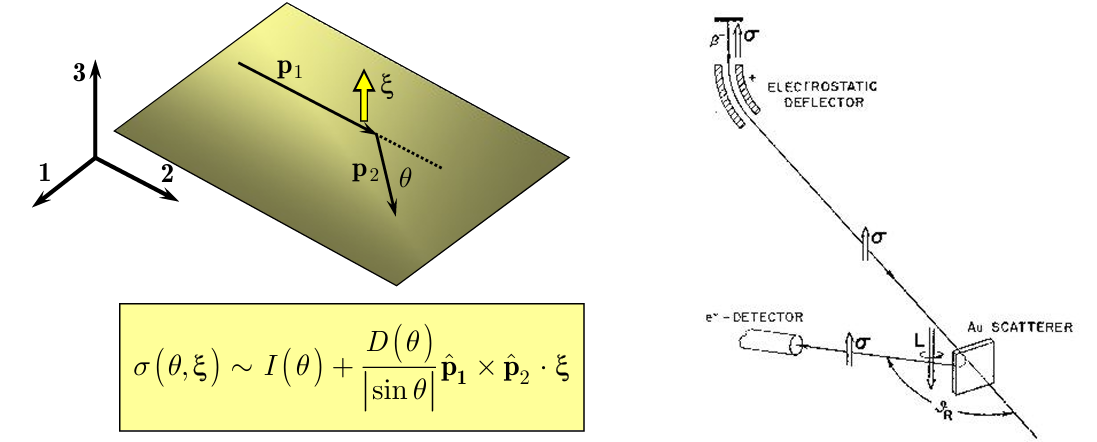
\includegraphics[width=0.8\textwidth]{Lezioni/Lezione 15/dra.png}
	\label{fig:dra}
\end{figure}
Notiamo che se l'angolo di deflessione $\theta$ va a sinistra il prodotto vettoriale $\hat{p}_1\times\hat{p}_2$ cambia segno (cambia il segno della componente $1$ di $p_2$)
$$
\left( \hat{\mathbf{p}}_1 \times \hat{\mathbf{p}}_2 \right)_3 = \varepsilon_{3jk} \hat{p}_1^j \hat{p}_2^k = \varepsilon_{321} \hat{p}_1^2 \hat{p}_2^1
$$
Supponiamo adesso che gli elettroni siano completamente polarizzati: in un caso paralleli alla quantità di moto ($RH$) e nell'altro caso antiparalleli ($LH$). Dopo la rotazione gli elettroni sono ancora completamente polarizzati. Nel primo caso verso l'alto nel secondo caso verso il basso. Guardando la formula della sezione d'urto assumiamo il piano $p_1-p_2$ perpendicolare a $\xi$. Le misure da fare sono:
\begin{figure}[h!]
	\centering
	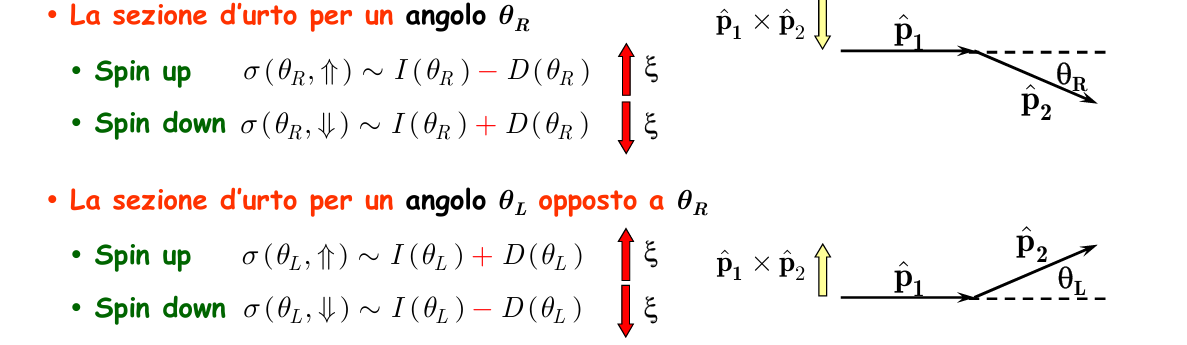
\includegraphics[width=0.6\textwidth]{Lezioni/Lezione 15/pro.png}
	\label{fig:pro}
\end{figure}
Nell'esperimento gli elettroni non sono completamente polarizzati. La misura della polarizzazione $\wp$ è l'obbiettivo dell'esperimento. La polarizzazione degli elettroni è data da 
$$
\wp = \frac{N_+ - N_-}{N_+ + N_-} \qquad N = N_+ + N_-
$$
Dove $N_+$ polarizzazione up e $N_-$ polarizzazione down. La sezione d'urto osservata per un angolo $\theta_R$ è
$$
\sigma(\theta_R) = \frac{N_+}{N}\sigma(\theta_R, \Uparrow) + \frac{N_-}{N}\sigma(\theta_R, \Downarrow) \qquad \sigma(\theta_R) \sim I(\theta_R) - \wp D(\theta_R)
$$
Analogamente, per un angolo $\theta_L$ si osserva
$$
\sigma(\theta_L) = \frac{N_+}{N}\sigma(\theta_L, \Uparrow) + \frac{N_-}{N}\sigma(\theta_L, \Downarrow) \qquad \sigma(\theta_L) \sim I(\theta_L) + \wp D(\theta_L)
$$
Definiamo l'assimetria $\delta$
$$
\delta = \frac{\sigma(\theta_L) - \sigma(\theta_R)}{\sigma(\theta_L) + \sigma(\theta_R)}
$$
Ci mettiamo nella condizione 
$$
\theta_R = -\theta_L \equiv \theta
$$
Si può verificare che
$$
I(\theta) = I(-\theta) \qquad D(\theta) = D(-\theta) \qquad \delta = \frac{D(\theta)}{I(\theta)}\wp \equiv S(\theta)\wp
$$
$S(\theta)$ è noto: la misura di $\delta$ permette di misurare $\wp$. Osservazioni: $S(\theta)$ dipende anche dall'energia dell'elettrone infatti è necessario che gli angoli $\theta_R$ e $\theta_L$ siano perfettamente simmetrici. L'esperimento è sensibile solo alla polarizzazione trasversale (un errore nella rotazione dello spin porta ad un errore sistematico su $\wp$). L'effetto aumenta al crescere di $Z$ e quindi si usano metalli pesanti come l'oro. Per ottimizzare l'esperimento si può cercare l'angolo al quale l'effetto è più grande. Occorre però tenere presente che al crescere dell'angolo la sezione d'urto diminuisce. Occorre trovare un compromesso tra la dimensione dell'effetto misurato e l'errore statistico con cui esso viene determinato. La tabella mostra i risultati del primo esperimento (con esperimenti successivi $\wp=-\beta_e$).
\begin{figure}[h!]
	\centering
	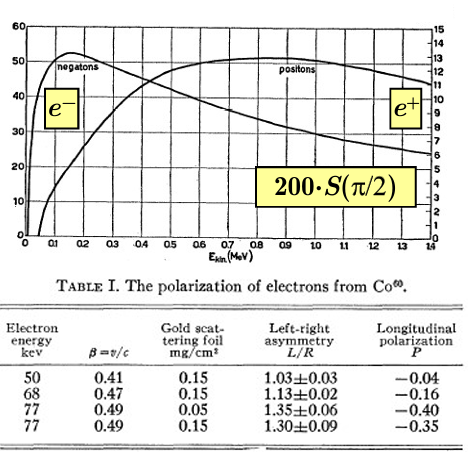
\includegraphics[width=0.6\textwidth]{Lezioni/Lezione 15/tab.png}
	\label{fig:tab}
\end{figure}
\section{Determinazione di $C_A$ e $C_V$}
Abbiamo già visto che la misura della vita media di nuclei permette di determinare la costante di accoppiamento $G_\beta$
$$
\lambda_F = \frac{1}{\tau} = \frac{G_\beta^2}{2\pi^3}\xi f
$$
Tuttavia, il parametro $\xi$ contiene una dipendenza dal rapporto $C_A/C_V$
$$
\xi = |\langle 1 \rangle|^2 + \frac{C_A^2}{C_V^2} |\langle \boldsymbol{\sigma} \rangle|^2
$$
I decadimenti di Fermi contengono solo il termine $<\mathbf{1}>$ e permettono pertanto la determinazione di $G_\beta^2$ senza ulteriori informazioni
$$
G_\beta = 1.13578 \pm 0.00027 \times 10^{-5} \, \text{GeV}^{-2}
$$
Ulteriori misure su transizioni di Gamov-Teller o miste permettono la determinazione di $|C_A/C_V|$
$$
\left| \frac{C_A}{C_V} \right| = 1.2695 \pm 0.0029
$$
Il segno relativo delle due costanti si può determinare solo con la misura di una grandezza osservabile che dipenda dal prodotto $C_A\cdot C_V$ e quindi dall'interferenza fra termini di Fermi e Gamov-Teller. Occorre pertanto studiare transizioni di nuclei polarizzati. Per nuclei non polarizzati l'elemento di matrice contiene il termine $1+\alpha\beta_e\cdot\beta_\nu$. Osservabili che dipendono dal vettore di polarizzazione del nucleo $\sigma$ contengono termini del tipo:
$$
1 + a\boldsymbol{\beta}_e \cdot \boldsymbol{\beta}_\nu + b\hat{\boldsymbol{\sigma}} \cdot \boldsymbol{\beta}_e + c\hat{\boldsymbol{\sigma}} \cdot \boldsymbol{\beta}_\nu
$$
Per neutroni polarizzati si trova
$$
b = -2 \frac{C_A^2 + C_V C_A}{C_V^2 + 3C_A^2} \qquad c = 2 \frac{C_A^2 - C_V C_A}{C_V^2 + 3C_A^2}
$$
Misure di correlazione angolare fra la direzione dell'elettrone (o del neutrino) e lo spin nucleare mostrano che il segno relativo è positivo
$$
\frac{C_A}{C_V} = +1.2695 \pm 0.0029
$$
\section{L'Hamiltoniana del Decadimento $\beta$}
Gli esperimenti hanno permesso la determinazione della forma dell'Hamiltoniana del decadimento $\beta$. Sono stati esclusi i termini Scalare e Tensoriale
$$
C_S = C_T = 0
$$
Sono state determinate le costanti degli accoppiamenti Vettoriale e Assiale
$$
G_\beta = G C_V \qquad \frac{C_A}{C_V} = \kappa \qquad \alpha_V = \alpha_A = 1
$$
L'Hamiltoniana pertanto contiene solo termini $V$ e $A$
$$
\mathcal{H}'_I = G \left[ C_V (\overline{\psi}_p \gamma^\mu \psi_n) (\overline{\psi}_e (1 + \gamma^5) \gamma_\mu \psi_\nu) + C_A (\overline{\psi}_p \gamma^5 \gamma^\mu \psi_n) (\overline{\psi}_e (1 + \gamma^5) \gamma^5 \gamma_\mu \psi_\nu) \right]
$$
Il termine assiale può essere semplificato utilizzando $(\gamma^5)^2=I$
$$
\mathcal{H}'_I = G \left[ C_V (\overline{\psi}_p \gamma^\mu \psi_n) (\overline{\psi}_e (1 + \gamma^5) \gamma_\mu \psi_\nu) + C_A (\overline{\psi}_p \gamma^5 \gamma^\mu \psi_n) (\overline{\psi}_e (1 + \gamma^5) \gamma_\mu \psi_\nu) \right]
$$
Infine raccogliamo la parte leptonica
$$
\mathcal{H}'_I = G \left[ C_V (\overline{\psi}_p \gamma^\mu \psi_n) + C_A (\overline{\psi}_p \gamma^5 \gamma^\mu \psi_n) \right] (\overline{\psi}_e (1 + \gamma^5) \gamma_\mu \psi_\nu)
$$
Possiamo ulteriormente semplificare
$$
\mathcal{H}'_I = G (\overline{\psi}_p (C_V + C_A \gamma^5) \gamma^\mu \psi_n) (\overline{\psi}_e (1 + \gamma^5) \gamma_\mu \psi_\nu)
$$
E ancora
$$
\mathcal{H}'_I = G C_V (\overline{\psi}_p (1 + \kappa \gamma^5) \gamma^\mu \psi_n) (\overline{\psi}_e (1 + \gamma^5) \gamma_\mu \psi_\nu)
$$
Come abbiamo già detto $\kappa=1.27$ e $GC_V\equiv G_\beta$. Il valore di $\kappa$ diverso da $1$ dipende dal fatto che il nucleone non è una particella puntiforme. Il protone ha una struttura ma ritorneremo su questo punto in seguito. Per il momento trascuriamo questo aspetto e assumiamo $\kappa=1$. Ciò risulta esatto per particelle puntiformi, ad esempio per i quark
$$
\mathcal{H}'_I = G_\beta \overline{\psi}_p (1 + \gamma^5) \gamma^\mu \psi_n \cdot \overline{\psi}_e (1 + \gamma^5) \gamma_\mu \psi_\nu
$$
In una notazione più moderna è diventato abituale spostare la matrice $\gamma^\mu$ a sinistra
$$
\mathcal{H}'_I = G_\beta \overline{\psi}_p \gamma^\mu (1 - \gamma^5) \psi_n \cdot \overline{\psi}_e \gamma_\mu (1 - \gamma^5) \psi_\nu
$$
Definiamo due generiche correnti (sia adronica che leptonica):
\begin{itemize}
	\item Una corrente Vettoriale: $J_V^\mu = \overline{\psi} \gamma^\mu \psi$
	\item Una corrente Assiale: $J_A^\mu = \overline{\psi} \gamma^\mu \gamma^5 \psi$
\end{itemize}
Le due correnti (adronica e leptonica) compaiono nell'Hamiltoniana nella combinazione
$$
J^\mu = J_V^\mu - J_A^\mu
$$
Ed è questa la famosa forma $V-A$ delle correnti deboli (cariche perché nella corrente cambia la carica!). Infine, per uniformarci alle notazioni maggiormente utilizzate ridefiniamo la costante di accoppiamento dell'interazione. La costante $G$ è stata definita da Fermi prima della scoperta della violazione di parità. La generalizzazione dell'interazione di Fermi e l'introduzione della violazione della parità hanno condotto ad una Hamiltoniana che contiene la differenza di due correnti ($V-A$). Per mantenere la stessa definizione di Fermi è necessario dividere $G$ per $\sqrt{2}$
$$
\mathcal{H}'_I = \frac{G_\beta}{\sqrt{2}} \overline{\psi}_p \gamma^\mu (1 - \gamma^5) \psi_n \cdot \overline{\psi}_e \gamma_\mu (1 - \gamma^5) \psi_\nu
$$
\section{Proiezioni chirali}
Esaminiamo in maggiore dettaglio la corrente leptonica
$$
l^\mu(x) = \overline{\psi}_e(x) \gamma^\mu (1 - \gamma^5) \psi_\nu(x)
$$
L'elemento di matrice di $l^\mu(0)$ fra il vuoto e lo stato $|e^-\overline{\nu}_e\rangle$ è
$$
\langle e^- \overline{\nu}_e | l^\mu(0) | 0 \rangle = \overline{u}_{p_e} \gamma^\mu (1 - \gamma^5) v_{p_\nu}
$$
Abbiamo già calcolato l'elemento di matrice di un operatore simile nel caso del decadimento $\beta$ ma vediamo ora le conseguenze della presenza della matrice $1-\gamma^5$. In particolare cosa implica per l'elettrone visto che nel decadimento $\beta$ gli elettroni sono polarizzati. Trasportiamo la matrice $1-\gamma^5$ a sinistra
$$
\overline{u}_{p_e} \gamma^\mu (1 - \gamma^5) v_{p_\nu} = \overline{u}_{p_e} (1 + \gamma^5) \gamma^\mu v_{p_\nu} = u_{p_e}^\dagger \gamma^0 (1 + \gamma^5) \gamma^\mu v_{p_\nu}
$$
$$
= u_{p_e}^\dagger (1 - \gamma^5) \gamma^0 \gamma^\mu v_{p_\nu} = [(1 - \gamma^5) u_{p_e}]^\dagger \gamma^0 \gamma^\mu v_{p_\nu} = \overline{[(1 - \gamma^5) u_{p_e}]} \gamma^\mu v_{p_\nu}
$$
Dimostriamo adesso che l'applicazione di $1-\gamma^5$ allo spinore $u(p)$ produce un elettrone con polarizzazione $\beta$ e che $\beta$ è la velocità dell'elettrone. Ricordiamo la definizione dell'operatore elicità
$$
\hat{h}(\hat{\mathbf{n}}) = \frac{\boldsymbol{\Sigma} \cdot \mathbf{p}}{|\mathbf{p}|} = \boldsymbol{\Sigma} \cdot \hat{\mathbf{n}} \qquad \hat{\mathbf{n}} = \frac{\mathbf{p}}{|\mathbf{p}|}
$$
Nel seguito utilizzeremo la rappresentazione di Dirac. In questa rappresentaizone l'operatore $\Sigma$ è
$$
\boldsymbol{\Sigma} = \begin{pmatrix} \boldsymbol{\sigma} & 0 \\ 0 & \boldsymbol{\sigma} \end{pmatrix}
$$
Consideriamo gli spinori $u_+$ e $u_-$
$$
u_+ = N \begin{pmatrix} \chi_+ \\ \frac{\boldsymbol{\sigma} \cdot \mathbf{p} \chi_+}{E + m} \end{pmatrix} = N \begin{pmatrix} \chi_+ \\ \frac{p \chi_+}{E + m} \end{pmatrix} \qquad u_- = N \begin{pmatrix} \chi_- \\ \frac{\boldsymbol{\sigma} \cdot \mathbf{p} \chi_-}{E + m} \end{pmatrix} = N \begin{pmatrix} \chi_- \\ \frac{-p \chi_-}{E + m} \end{pmatrix} \qquad N = \sqrt{E + m}
$$
$\chi_\pm$ sono spinori bidimensionali autovettori di $\sigma\cdot\hat{n}$ e si verifica facilmente che gli spinori $u_\pm$ sono autostati dell'elicità
$$
\boldsymbol{\sigma} \cdot \hat{\mathbf{n}} \chi_\pm = \pm \chi_\pm
$$
Infatti
$$
\boldsymbol{\Sigma} \cdot \hat{\mathbf{n}} u_+ = \begin{pmatrix} \boldsymbol{\sigma} \cdot \hat{\mathbf{n}} & 0 \\ 0 & \boldsymbol{\sigma} \cdot \hat{\mathbf{n}} \end{pmatrix} N \begin{pmatrix} \chi_+ \\ \frac{p \chi_+}{E + m} \end{pmatrix} = N \begin{pmatrix} \boldsymbol{\sigma} \cdot \hat{\mathbf{n}} \chi_+ \\ \frac{p \boldsymbol{\sigma} \cdot \hat{\mathbf{n}} \chi_+}{E + m} \end{pmatrix} = +N \begin{pmatrix} \chi_+ \\ \frac{p \chi_+}{E + m} \end{pmatrix}
$$
$$
\boldsymbol{\Sigma} \cdot \hat{\mathbf{n}} u_+ = +u_+ \qquad \boldsymbol{\Sigma} \cdot \hat{\mathbf{n}} u_- = -u_-
$$
In definitiva, per $\lambda=\pm 1$
$$
\boldsymbol{\Sigma} \cdot \hat{\mathbf{n}} u_\lambda = \lambda u_\lambda
$$
Il risultato precedente significa che $u_\pm$ rappresentano spinori completamente polarizzati lungo la direzione del moto ($\wp=100\%$):
\begin{itemize}
	\item $u_+$ è uno spinore con polarizzazione $100\%$ in direzione parallela a $p$
	\item $u_-$ è uno spinore con polarizzazione $100\%$ in direzione antiparallela a $p$
\end{itemize}
Consideriamo adesso un arbitrario spinore nella rappresentazione di Dirac (non necessariamente normalizzato)
$$
u(p) = N \begin{pmatrix} \chi \\ \frac{\boldsymbol{\sigma} \cdot \mathbf{p} \chi}{E + m} \end{pmatrix}
$$
$$
u_R = \frac{1}{2}(1 + \gamma^5) u \qquad u_L = \frac{1}{2}(1 - \gamma^5) u
$$
Definiamo le proiezioni chirali $u_R$ e $u_L$ ricordando che la formua di $\gamma^5$ nella rappresentazione di Dirac è
$$
\gamma^5 = \begin{pmatrix} 0 & I \\ I & 0 \end{pmatrix} \qquad 1 - \gamma^5 = \begin{pmatrix} I & -I \\ -I & I \end{pmatrix} \qquad 1 + \gamma^5 = \begin{pmatrix} I & I \\ I & I \end{pmatrix}
$$
Otteniamo
$$
u_L = \frac{1}{2}(1 - \gamma^5) u(p) = \frac{N}{2} \begin{pmatrix} I & -I \\ -I & I \end{pmatrix} \begin{pmatrix} \chi \\ \frac{\boldsymbol{\sigma} \cdot \mathbf{p} \chi}{E + m} \end{pmatrix} = \frac{N}{2} \begin{pmatrix} \left(1 - \frac{\boldsymbol{\sigma} \cdot \mathbf{p}}{E + m}\right) \chi \\ -\left(1 - \frac{\boldsymbol{\sigma} \cdot \mathbf{p}}{E + m}\right) \chi \end{pmatrix}
$$
Notiamo che le componenti superiori dello spinore e quelle inferiori non sono più indipendenti. Quindi questa proiezione rimuove dei gradi di libertà allo spinore. Osserviamo inoltre che lo spinore $u_L$ non è un autostato dell'operatore elicità $h$ tuttavia, si può verificare esplicitamente che il valore medio dell'elicità è
$$
\langle h \rangle_L = \frac{\langle u_L | \hat{h} | u_L \rangle}{\langle u_L | u_L \rangle} = - \frac{p}{E} = -\beta
$$
Quindi lo stato non è polarizzato al $100\%$ come $u_{\pm}$ in quanto $\beta<1$! Quindi l'effetto di quel proiettore che abbiamo introdotto dal punto di vista cinematico introduce esattamente la cosa che abbiamo osservata cioè la violazione di parità dalla polarizzazione degli elettroni.
Consideriamo adesso $u_R$
$$
u_R = \frac{1}{2}(1 + \gamma^5) u(p) = \begin{pmatrix} I & I \\ I & I \end{pmatrix} \begin{pmatrix} \chi \\ \frac{\boldsymbol{\sigma} \cdot \mathbf{p}\chi}{E + m} \end{pmatrix} = \begin{pmatrix} \left(1 + \frac{\boldsymbol{\sigma} \cdot \mathbf{p}}{E + m}\right)\chi \\ \left(1 + \frac{\boldsymbol{\sigma} \cdot \mathbf{p}}{E + m}\right)\chi \end{pmatrix}
$$
Analogamente al caso precedente si può verificare che
$$
\langle h \rangle_R = \frac{\langle u_R | \hat{h} | u_R \rangle}{\langle u_R | u_R \rangle} = + \frac{p}{E} = +\beta
$$
Pertanto gli spinori $u_L$ e $u_R$ non sono autostati dell'operatore elicità tuttavia rappresentano stati con polarizzazione parziale $\wp=\pm\beta$. Notiamo infine che per $\beta\to1$ la polarizzazione diventa completa e le due proiezioni chirali diventano autostati dell'elicità. Abbiamo pertanto ritrovato il risultato sulla polarizzazione $\beta$ che avevamo ottenuto precedentemente con il calcolo esplicito dell'elemento di matrice. Possiamo vedere una ulteriore motivazione per la polarizzazione degli elettroni come il risultato della struttura $V-A$ della corrente leptonica. L'operatore $1-\gamma^5$ proietta uno spinore arbitrario in uno stato di polarizzazione parziale longitudinale left-handed. Ribadiamo inoltre che la polarizzazione diventa completa quanto $\beta\to 1$. Le notazioni $u_R$ e $u_L$ per indicare le proiezioni chirali possono generare confusione ed è per questo che bisogna tenere distinti i concetti di chiralità e elicità. L'Hamiltoniana delle interazioni debole contiene le proiezioni chirali. Ritorneremo su questo punto.
\section{Rappresentazione Chirale delle matrici $\gamma$}
La rappresentazione di Dirac delle matrici $\gamma$ è stata utile per discutere il limite non relativistico dell'equazione di Dirac (comoda perché si separato le due componenti large e small). Se si vogliono mettere in evidenza altri aspetti sono più convenienti altre rappresentazioni. Ad esempio il limite di alta energia o, equivalentemente, il limite di massa nulla. Aspetti legati alla handedness o Chiralità. In questi casi è conveniente la rappresentazione Chirale o di Weyl
$$
\boldsymbol{\alpha} = \begin{pmatrix} \boldsymbol{\sigma} & \mathbf{0} \\ \mathbf{0} & -\boldsymbol{\sigma} \end{pmatrix} \qquad \beta = \gamma^0 = \begin{pmatrix} 0 & I \\ I & 0 \end{pmatrix} \qquad \boldsymbol{\gamma} = \gamma^0\boldsymbol{\alpha} = \begin{pmatrix} 0 & -\boldsymbol{\sigma} \\ \boldsymbol{\sigma} & 0 \end{pmatrix} \qquad \gamma^5 = \begin{pmatrix} I & 0 \\ 0 & -I \end{pmatrix}
$$
$$
\boldsymbol{\alpha}\gamma^5 = \gamma^5\boldsymbol{\alpha} = \boldsymbol{\Sigma} = \begin{pmatrix} \boldsymbol{\sigma} & \mathbf{0} \\ \mathbf{0} & \boldsymbol{\sigma} \end{pmatrix} \qquad \frac{1}{2}(1 + \gamma^5) = \begin{pmatrix} I & \mathbf{0} \\ \mathbf{0} & \mathbf{0} \end{pmatrix} \qquad \frac{1}{2}(1 - \gamma^5) = \begin{pmatrix} \mathbf{0} & \mathbf{0} \\ \mathbf{0} & I \end{pmatrix}
$$
Nella rappresentazione di Weyl si separano le proiezioni chirali $R$ e $L$ degli spinori. Nella rappresentazione di Dirac si separano le componenti Large o Small legate al limite non relativistico. Studiamo l'equazione di Dirac nella rappresentazione chirale
$$
(\boldsymbol{\alpha} \cdot \mathbf{p} + \beta m)\psi = E\psi
$$
Utilizziamo la rappresentazione chirale e la rappresentazione a blocchi dello spinore
$$
\psi = \begin{pmatrix} \chi \\ \phi \end{pmatrix}
$$
L'equazione diventa
$$
\begin{pmatrix} \boldsymbol{\sigma} \cdot \mathbf{p} & \mathbf{0} \\ \mathbf{0} & -\boldsymbol{\sigma} \cdot \mathbf{p} \end{pmatrix} \begin{pmatrix} \chi \\ \phi \end{pmatrix} - E \begin{pmatrix} \chi \\ \phi \end{pmatrix} = -m \begin{pmatrix} 0 & I \\ I & 0 \end{pmatrix} \begin{pmatrix} \chi \\ \phi \end{pmatrix}
$$
L'equazione matriciale corrisponde alle due equazioni accoppiate
$$
\boldsymbol{\sigma} \cdot \mathbf{p}\chi - E\chi = -m\phi \qquad \boldsymbol{\sigma} \cdot \mathbf{p}\phi + E\phi = +m\chi
$$
Nella rappresentazione di Dirac avevamo trovato
$$
\boldsymbol{\sigma} \cdot \mathbf{p}\phi - E\chi = -m\chi \qquad \boldsymbol{\sigma} \cdot \mathbf{p}\chi - E\phi = +m\phi
$$
Notiamo un aspetto interessante del limite di massa nulla $m=0$. Nella rappresentazione di Weyle le equazioni per $\chi$ e $\phi$ si disaccoppiano. Nella rappresentazione di Dirac le due equazioni rimangono accoppiate anche nel caso limite di massa nulla. Nel caso di massa nulla le equazioni diventano ($E=|\mathbf{p}|=\mathbf{p}$, $\hat{\mathbf{p}}=\mathbf{p}/p$)
$$
\boldsymbol{\sigma} \cdot \mathbf{p}\chi - E\chi = 0 \implies \boldsymbol{\sigma} \cdot \hat{\mathbf{p}}\chi = +\chi
$$
$$
\boldsymbol{\sigma} \cdot \mathbf{p}\phi + E\phi = 0 \implies \boldsymbol{\sigma} \cdot \hat{\mathbf{p}}\phi = -\phi
$$
Vediamo pertanto che i due spinori bidimensionali $\chi$ e $\phi$ sono autostati dell'elicità. Inoltre nella rappresentazione chirale i due operatori di proiezione sono
$$
\frac{1}{2}(1 - \gamma^5) = \frac{1}{2} \left[ \begin{pmatrix} I & 0 \\ 0 & I \end{pmatrix} - \begin{pmatrix} I & 0 \\ 0 & -I \end{pmatrix} \right] = \begin{pmatrix} 0 & 0 \\ 0 & I \end{pmatrix} \quad \frac{1}{2}(1 + \gamma^5) = \begin{pmatrix} I & 0 \\ 0 & 0 \end{pmatrix}
$$
Applicando i due opertori allo spinore generico
$$
\psi = \begin{pmatrix} \chi \\ \phi \end{pmatrix} \qquad \psi_R = \frac{1}{2}(1 + \gamma^5)\psi = \begin{pmatrix} \chi \\ 0 \end{pmatrix} \qquad \psi_L = \frac{1}{2}(1 - \gamma^5)\psi = \begin{pmatrix} 0 \\ \phi \end{pmatrix}
$$ 
Notiamo infine che i due spinori $\psi_L$ e $\psi_R$ sono anche autovettori dell'operatore $\gamma^5$ (operatore chiralità) con autovalori $+1$ e $-1$
$$
\gamma^5 \psi_R = +\psi_R \qquad \gamma^5 \psi_L = -\psi_L
$$
Abbiamo già notato che per $m=0$ chiralità ed elicità coincidono. Per una massa non nulla sono due proprietà differenti: Elicità $\to$ polarizzazione completa; Chiralità $\to$ polarizzazione parziale $\wp=\beta$. La separazione delle due componenti è specifica delle rappresentazioni chirali. Tuttavia molde delle altre proprietà viste sono indipendenti dalla massa e dalla rappresentazione. Consideriamo ancora i due proiettori
$$
\hat{P}_R = \frac{1}{2}(1 + \gamma^5) \qquad \hat{P}_L = \frac{1}{2}(1 - \gamma^5) \qquad \hat{P}_R \hat{P}_L = 0 \qquad \hat{P}_R + \hat{P}_L = \hat{I}
$$
Si può sempre scomporre uno spinore in due componenti chirali $\psi=\psi_L+\psi_R$
$$
\psi = \psi_L + \psi_R \qquad \psi_R = \frac{1}{2}(1 + \gamma^5)\psi = \hat{P}_R \psi \qquad \psi_L = \frac{1}{2}(1 - \gamma^5)\psi = \hat{P}_L \psi
$$
Le due componenti chirali di $\psi$ sono autovettori di $\gamma^5$
$$
\gamma^5 \psi_R = \frac{1}{2}\gamma^5(1 + \gamma^5)\psi = \frac{1}{2}(\gamma^5 + 1)\psi = +\psi_R
$$
$$
\gamma^5 \psi_L = \frac{1}{2}\gamma^5(1 - \gamma^5)\psi = \frac{1}{2}(\gamma^5 - 1)\psi = -\psi_L
$$
In generale le due componenti non sono soluzioni dell'equazione di Dirac. Osserviamo che, dato che $$
\{\gamma^5, \gamma^\mu\} = 0, \qquad \hat{P}_R \gamma^\mu = \gamma^\mu \hat{P}_L \quad \text{e} \quad \hat{P}_L \gamma^\mu = \gamma^\mu \hat{P}_R
$$
Pertanto se
$$
(\slashed{p} - m)\psi = 0 \implies (\slashed{p} - m)\psi_R = (\slashed{p} - m)\hat{P}_R \psi = (\hat{P}_L \slashed{p} - \hat{P}_R m)\psi \neq 0
$$
Analogamente per l'altra componente. Tuttavia se $m=0$ le due componenti sono soluzioni dell'equazione di Dirac
$$
\slashed{p}\psi = 0 \qquad \implies \qquad \slashed{p}\psi_R = \slashed{p}\hat{P}_R \psi = \hat{P}_L \slashed{p}\psi = 0
$$
\subsection{Proiezioni chirali e antiparticelle}
Discutiamo adesso le proiezioni chirali degli spinori $v$ associati alle soluzioni con energia negativa. Abbiamo già notato che l'associazione dell'elicità fisica $+1$ agli autovalori dell'operatore $\Sigma\cdot\mathbf{p}$ è opposta a quella degli spinori $u$. Va comunque ricordato che la polarizzazione calcolata con l'elemento di matrice ha sempre il segno corretto, sia che si producano particelle o antiparticelle. I proiettori di spin covarianti sono stati costruiti in modo da tenere conto dell'inversione di segno. Analogamente a questo succede per l'elicità risulta anche invertito il segno della polarizzazione associata alle proiezioni chirali $L$ e $R$. Questo aspetto è evidente nel caso di particelle di massa nulla. Consideriamo ancora l'equazione di Dirac nella rappresentazione chirale
$$
\boldsymbol{\sigma} \cdot \mathbf{p}\chi - p_0\chi = 0 \qquad \boldsymbol{\sigma} \cdot \mathbf{p}\phi + p_0\phi = 0
$$
nel caso di soluzioni con energia negativa $p_0=-E$
$$
\boldsymbol{\sigma} \cdot \mathbf{p}\chi + E\chi = 0 \qquad \boldsymbol{\sigma} \cdot \mathbf{p}\phi - E\phi = 0
$$
Pertanto, per le soluzioni di energia negativa, le relazioni diventano
$$
\boldsymbol{\sigma} \cdot \hat{\mathbf{p}}\chi = -\chi \qquad \boldsymbol{\sigma} \cdot \hat{\mathbf{p}}\phi = +\phi
$$
Per le antiparticelle l'elicità delle proiezioni (spinori $\chi$ e $\phi$) è scambiata. La conseguenza fisica di quanto detto è che nel decadimento $\beta$ le particelle sono emesse con polarizzazione $-\beta$ (ad esempio l'elettrone) mentre le antiparticelle sono emesse con polarizzazione $+\beta$ (ad esempio il neutrino). Per finire osserviamo che nel decadimento $\beta$ l'elicità dell'antineutrino è sempre right-handed. Ricordiamo l'elemento di matrice
$$
\langle e^- \overline{\nu}_e | l^\mu (0) | 0 \rangle = \overline{u}_{p_e} \gamma^\mu (1 - \gamma^5) v_{p_\nu}
$$
Lo spinore $v$ si può scomporre
$$
v = v_L + v_R = \frac{1}{2}(1 - \gamma^5)v + \frac{1}{2}(1 + \gamma^5)v
$$
Calcoliamo l'effetto dell'operatore $1-\gamma^5$ presente nell'elemento di matrice
$$
(1 - \gamma^5)v = (1 - \gamma^5) \left[ \frac{1}{2}(1 + \gamma^5) + \frac{1}{2}(1 - \gamma^5) \right] v
$$
$$
= \frac{1}{2}(1 - \gamma^5)(1 - \gamma^5)v + \frac{1}{2}(1 - \gamma^5)(1 + \gamma^5)v = (1 - \gamma^5)v_L
$$
Pertanto nel decadimento $\beta$ l'elicità dell'antineutrino è sempre $RH$ mentre l'elicità del neutrino è sempre $LH$. Allora è nata la domanda: la componente $RH$ del neutrino non ha interazione elettromagnetico perché neutro, non ha interazione forte perché è un leptone non ha interazione debole perchè è $RH$ con chi interagisce? non ha massa non ha interazione gravitazionale allora forse non esiste. Allora è nata una teoria che giustificava la violazione della parità con il fatto che il neutrino era una particella con solo due gradi di libertà e non quattro. Questa cosa ancora non è del tutto chiarita. Questo perchè se da un lato il neutrino ha effettivamente una massa però è estremamente piccola quindi anche se $\beta$ non è esattamente $1$ la probabilità di vedere questi neutrini è comunque super infinitesima. Rimane il quesito se i neutrini sono particelle di Dirac con $4$ gradi di libertà o particelle di Majorana con $2$ gradi di libertà (particelle che coincidono con le proprie antiparticelle - esperimenti per misurare i decadimenti doppi $\beta$ -).
\section{Violazione della parità e momento angolare}
Abbiamo visto che la presenza dell'operatore $1-\gamma^5$ determina una polarizzazione nei leptoni prodotti nel decadimento $\beta$. Fermioni left-handed e anti-fermioni right-handed. Questa circostanza ci permette di dare un'interpretazione interessate dei risultati sulle correlazioni angolari del decadimento $\beta$: $n\to p+e^-+\overline{\nu}_e$. La correlazione angolare è una conseguenza della conservazione della conservazione del momento angolare e dal fatto che i due leptoni sono polarizzati. Abbiamo infatti visto che le transizioni di Fermi non cambiano il momento angolare del nucleo. I leptoni pertanto sono in uno stato di singoletto e il momento angolare emesso è $S=0$ ($\cos(\theta_{e\nu})\sim -1$). Per le transizioni di Gamov-Teller invece il momento angolare nucleare varia di una unità. I leptoni sono adesso in uno stato di tripletto e il momento angolare è $S=1$ ($\cos(\theta_{e\nu})\sim -1$).
\subsection{Le correnti chirali left-handed}
Ci sono altre osservazioni che si possono fare sulla corrente
$$
J^\mu = \overline{\psi}_a \gamma^\mu (1 - \gamma^5) \psi_b
$$
Osserviamo che
$$
\frac{1}{2}(1 - \gamma^5)\frac{1}{2}(1 - \gamma^5) = \frac{1}{4}(1 - 2\gamma^5 + (\gamma^5)^2) = \frac{1}{4}(2 - 2\gamma^5) = \frac{1}{2}(1 - \gamma^5)
$$
$$
\frac{1}{2}(1 - \gamma^5)\frac{1}{2}(1 - \gamma^5) = \frac{1}{2}(1 - \gamma^5)
$$
Possiamo pertanto scrivere
$$
\overline{\psi}_a \gamma^\mu (1 - \gamma^5) \psi_b = 2\overline{\psi}_a \gamma^\mu \frac{1}{2}(1 - \gamma^5) \psi_b = 2\overline{\psi}_a \gamma^\mu \frac{1}{2}(1 - \gamma^5) \frac{1}{2}(1 - \gamma^5) \psi_b
$$
$$
= 2\overline{\psi}_a \frac{1}{2}(1 + \gamma^5) \gamma^\mu \frac{1}{2}(1 - \gamma^5) \psi_b = 2\psi_a^\dagger \gamma^0 \frac{1}{2}(1 + \gamma^5) \gamma^\mu \frac{1}{2}(1 - \gamma^5) \psi_b
$$
$$
= 2\psi_a^\dagger \frac{1}{2}(1 - \gamma^5) \gamma^0 \gamma^\mu \frac{1}{2}(1 - \gamma^5) \psi_b = 2 \left[ \frac{1}{2}(1 - \gamma^5) \psi_a \right]^\dagger \gamma^0 \gamma^\mu \frac{1}{2}(1 - \gamma^5) \psi_b
$$
$$
J^\mu = 2 \left[ \frac{1}{2} (1 - \gamma^5) \psi_a \right]^\dagger \gamma^0 \gamma^\mu \frac{1}{2} (1 - \gamma^5) \psi_b
$$
Introduciamo le proiezioni chirali Left degli operatori di campo
$$
\psi_L = \frac{1}{2} (1 - \gamma^5) \psi
$$
Inserendo nella corrente abbiamo
$$
J^\mu = 2 [\psi_{aL}]^\dagger \gamma^0 \gamma^\mu \psi_{bL} = 2 \overline{\psi}_{aL} \gamma^\mu \psi_{bL} \qquad J^\mu = 2 \overline{\psi}_{aL} \gamma^\mu \psi_{bL}
$$
Pertanto un altro modo di sintetizzare i risultati sperimentali sui decadimenti deboli è: solo le proiezioni chirali Left dei fermioni partecipano ai decadimento deboli (chiralità non elicità). Attensione, solo per le correnti cariche mediate dai bosoni $W^{\pm}$. Nel modello standard questa affermazione si traduce nel limitare il gruppo di simmetria $SU(2)$ dell'isospin debole alle componenti $LH$ dei campi ($SU(2)_L$)